% Options for packages loaded elsewhere
\PassOptionsToPackage{unicode}{hyperref}
\PassOptionsToPackage{hyphens}{url}
%
\documentclass[
]{article}
\usepackage{lmodern}
\usepackage{amssymb,amsmath}
\usepackage{ifxetex,ifluatex}
\ifnum 0\ifxetex 1\fi\ifluatex 1\fi=0 % if pdftex
  \usepackage[T1]{fontenc}
  \usepackage[utf8]{inputenc}
  \usepackage{textcomp} % provide euro and other symbols
\else % if luatex or xetex
  \usepackage{unicode-math}
  \defaultfontfeatures{Scale=MatchLowercase}
  \defaultfontfeatures[\rmfamily]{Ligatures=TeX,Scale=1}
\fi
% Use upquote if available, for straight quotes in verbatim environments
\IfFileExists{upquote.sty}{\usepackage{upquote}}{}
\IfFileExists{microtype.sty}{% use microtype if available
  \usepackage[]{microtype}
  \UseMicrotypeSet[protrusion]{basicmath} % disable protrusion for tt fonts
}{}
\makeatletter
\@ifundefined{KOMAClassName}{% if non-KOMA class
  \IfFileExists{parskip.sty}{%
    \usepackage{parskip}
  }{% else
    \setlength{\parindent}{0pt}
    \setlength{\parskip}{6pt plus 2pt minus 1pt}}
}{% if KOMA class
  \KOMAoptions{parskip=half}}
\makeatother
\usepackage{xcolor}
\IfFileExists{xurl.sty}{\usepackage{xurl}}{} % add URL line breaks if available
\IfFileExists{bookmark.sty}{\usepackage{bookmark}}{\usepackage{hyperref}}
\hypersetup{
  pdftitle={Short Paper},
  hidelinks,
  pdfcreator={LaTeX via pandoc}}
\urlstyle{same} % disable monospaced font for URLs
\usepackage[margin=2cm]{geometry}
\usepackage{graphicx,grffile}
\makeatletter
\def\maxwidth{\ifdim\Gin@nat@width>\linewidth\linewidth\else\Gin@nat@width\fi}
\def\maxheight{\ifdim\Gin@nat@height>\textheight\textheight\else\Gin@nat@height\fi}
\makeatother
% Scale images if necessary, so that they will not overflow the page
% margins by default, and it is still possible to overwrite the defaults
% using explicit options in \includegraphics[width, height, ...]{}
\setkeys{Gin}{width=\maxwidth,height=\maxheight,keepaspectratio}
% Set default figure placement to htbp
\makeatletter
\def\fps@figure{htbp}
\makeatother
\setlength{\emergencystretch}{3em} % prevent overfull lines
\providecommand{\tightlist}{%
  \setlength{\itemsep}{0pt}\setlength{\parskip}{0pt}}
\setcounter{secnumdepth}{5}
\usepackage{subcaption}
\usepackage{longtable}

\title{Short Paper}
\author{true \and true \and true \and true}
\date{2020-10-30}

\begin{document}
\maketitle
\begin{abstract}
This is the abstract.
\end{abstract}

\hypertarget{introduction}{%
\section{Introduction}\label{introduction}}

Lorem ipsum dolor sit amet, consectetur adipiscing elit, sed do eiusmod
tempor incididunt ut labore et dolore magna aliqua. Ut enim ad minim
veniam, quis nostrud exercitation ullamco laboris nisi ut aliquip ex ea
commodo consequat. Duis aute irure dolor in reprehenderit in voluptate
velit esse cillum dolore eu fugiat nulla pariatur. Excepteur sint
occaecat cupidatat non proident, sunt in culpa qui officia deserunt
mollit anim id est laborum.Lorem ipsum dolor sit amet, consectetur
adipiscing elit, sed do eiusmod tempor incididunt ut labore et dolore
magna aliqua. Ut enim ad minim veniam, quis nostrud exercitation ullamco
laboris nisi ut aliquip ex ea commodo consequat. Duis aute irure dolor
in reprehenderit in voluptate velit esse cillum dolore eu fugiat nulla
pariatur. Excepteur sint occaecat cupidatat non proident, sunt in culpa
qui officia deserunt mollit anim id est laborum.Lorem ipsum dolor sit
amet, consectetur adipiscing elit, sed do eiusmod tempor incididunt ut
labore et dolore magna aliqua. Ut enim ad minim veniam, quis nostrud
exercitation ullamco laboris nisi ut aliquip ex ea commodo consequat.
Duis aute irure dolor in reprehenderit in voluptate velit esse cillum
dolore eu fugiat nulla pariatur. Excepteur sint occaecat cupidatat non
proident, sunt in culpa qui officia deserunt mollit anim id est laborum.

\hypertarget{background}{%
\section{Background}\label{background}}

\hypertarget{what-affects-the-decision-to-cycle}{%
\subsection{What Affects the Decision To
Cycle}\label{what-affects-the-decision-to-cycle}}

Segregated cycling
infrastructure\footnote{Segregated cycling infrastructure refers to road space that is allocated to cyclists only, with physical separation to protect cyclists from other modes of transport.}
has been shown to increase cycling uptake (Aldred et al., 2019; Goodman
et al., 2014; Marqués et al., 2015), with the separation from motorized
vehicles being key (Winters et al., 2011). Revealed preference of
cyclists shows that they are willing to deviate from the most efficient
routes in order to commute on safer roads (Crane et al., 2017). However,
such deviations are only considered if they do not considerably increase
route circuitry; behaviour studies have found that the probability of
choosing a route decreases in proportion to its length relative to the
shortest route (Broach et al., 2011; Winters et al., 2010). Another
defining feature for cycling infrastructure is how well connected it is.
Cyclists prefer cohesive infrastructure, particularly when cycling on
arterial roads with high levels of motorized traffic (Stinson and Bhat,
2003), and the lack of well-connected cycling infrastructure is one of
the main obstacles to increasing cycling uptake (Caulfield et al.,
2012). While direct and cohesive cycling networks have been shown to
positively impact cycling rates,
density\footnote{making an area's bicycle network denser means adding more cycling routes in the area and thereby giving cyclists more route options}
of the cycling network is also vital (Schoner and Levinson, 2014).

\hypertarget{planning-cycling-networks}{%
\subsection{Planning Cycling Networks}\label{planning-cycling-networks}}

\emph{Optimization} techniques have been used to propose improvements to
cycling networks. Mesbah et al. (2012) propose a bi-level formulation to
optimize allocation of cycling lanes to the network without exceeding a
set budget. The upper level is the proposed interventions and the lower
level is the route choices made by users in reaction to changes in the
network. The problem accounts for the effect of cycling lanes on car
traffic, and attempts to maximize utilization of said lanes with minimal
impact on car travel times. To improve cohesion of the suggested
network, a constraint is added so that each link with a bike lane should
be connected to at least one destination. Car usage is not considered by
Mauttone et al. (2017), who develop an optimization framework that aims
to minimize the total user cost of cycling on the network. The aggregate
flow on links is obtained by using shortest paths to route existing
cycling demand onto the road network, and the solution is a proposed set
of links where cycling infrastructure should be added in order to
minimize the overall travel cost of cyclists across the network. The
cost of traversing a link is given as a function of its length and
whether or not it has cycling infrastructure, and a discontinuity
penalty is also added to prioritize connected road segments. The problem
has also been solved by attempting to find the minimum cost of improving
roadway links to meet a desired level of service (LOS) (Duthie and
Unnikrishnan, 2014). In this formulation, all OD pairs need to be
connected by roads that meet the desired LOS, and a directness
constraint is added so that paths between OD pairs do not exceed a
certain multiple of the shortest path.

\vspace{0.3cm}

These problem formulations do not explicitly solve for continuity, which
is dealt with using a either (a) a constraint specifying that each link
with a bike lane should be connected to at least one destination (Mesbah
et al., 2012), (b) a constraint on deviation from shortest paths (Duthie
and Unnikrishnan, 2014), or (c) a discontinuity penalty (Mauttone et
al., 2017). To solve for continuity, the graph-theoretic concept of
\emph{connected components}, has been used. Natera et al. (2019) study
the existing cycling network in terms of its disconnected components and
introduce two different algorithms to connect these components by their
most critical
links\footnote{\textit{link} refers to a road segment throughout this research}
and, in doing so, measure the size of the growth of the largest
connected component as a function of the kilometers of network added.
They observe that small investments at strategic points have a large
impact on connectivity in most cases. The concept of connected
components is also at the core of the methodology proposed by Olmos et
al. (2020). After routing the cycling demand onto the network links,
they use percolation theory to filter out the links based on the
aggregate
flow\footnote{\textit{flow} is used throughout this research to refer to the cycling demand when it is routed onto the road network. The flow on any road segment is the cumulative demand on it, resulting from cyclists commuting between various OD pairs}
passing through them. They vary the flow threshold for filtering to
identify the minimum flow at which the whole city is connected by a
giant component. The results show a cycling network that connects the
entire city, and subtracting links intersecting with current cycling
infrastructure identifies links proposed for intervention.

\vspace{0.3cm}

The problem formulations outlined above look at the network as a whole
when attempting to improve it. An alternative approach is to identify
the different sub-networks that exist within the larger network, and
work on improving each separately. Trip patterns in a city are not
uniformly distributed geographically, and \emph{community finding}
methods have been used to partition study areas into localized areas
that experience a disproportionate number of trips within them.
Akbarzadeh et al. (2018) use a modularity maximization approach (Blondel
et al., 2008) on taxi trip data to identify 7 different communities in
the city of Isfahan, Iran. An optimization problem is then formulated to
connect nodes within each community with cycling infrastructure. The
emphasis is on connectivity within the communities, not between them.
Bao et al. (2017) adopt a similar methodology, but use hierarchical
clustering to specify the desired number of clusters. They use a greedy
network expansion algorithm, where the link with the highest
benefit/cost ratio in each cluster is selected, and the network is grown
by adding neighboring links to the solution until a budget limit is met.
The benefit is the flow on the link, and each link is assigned a cost
based on current road conditions.

\hypertarget{underlying-ethical-principles}{%
\subsection{Underlying Ethical
Principles}\label{underlying-ethical-principles}}

The methodologies in Section \textbf{How do I cite a section??} are
underpinned by different ethical principles, even though these
principles are not explicitly acknowledged by the authors. This is
important since different ethical principles constitute different
problem formulations and targets. Broadly speaking, transport appraisal
can be based on either utilitarian or egalitarian principles. The former
seeks to maximize the overall benefit, while the latter is concerned
with a fair distribution of benefits (Jafino et al., 2020).
Nahmias-Biran et al. (2017) criticize the utilitarian approach that has
been historically popular in the evaluation of transport investments,
explaining how the maximization of overall benefit fails to account for
the distribution of that benefit among communities or individuals. Lucas
et al. (2016) explain how transport studies have traditionally looked at
the bigger picture without studying the distribution of investments on
the different parts of the study area, and go on to propose an
egalitarian approach that ensures the dis-aggregation of transport
policy benefits across the study area. Pereira et al. (2017) also
emphasize the need for a more egalitarian approach to transport
planning. They highlight accessibility as a cornerstone of distributive
justice, and contend that policies should aim to distribute investments
in a way that minimizes spatial variations in accessibility. This
research attempts to provide a methodology that is grounded in
egalitarian principles. \textbf{Write some more here}

\hypertarget{data-and-geographical-scale-of-analysis}{%
\section{Data and Geographical Scale of
Analysis}\label{data-and-geographical-scale-of-analysis}}

The analysis is heavily dependant on Origin-Destination census data
(commuter data). Commuter data in the UK is publicly available at the
Middle layer Super Output Area (MSOA) level; the average MSOA has a
population of 8209 (ONS, 2018). Iacono et al. (2010) note that such
large travel zones are not ideal for understanding route choice
behaviour of cyclists and pedestrians. They also give rise to an
`ecological fallacy' whereby average characteristics are assumed to
apply to all residents of the aggregated geographical area. Given that
more granular data is not publicly available, the study uses MSOA-level
commuter data. The methodology is however applicable to more granular
commuter data should it become available.

\hypertarget{calculating-potential-cycling-demand}{%
\section{Calculating Potential Cycling
Demand}\label{calculating-potential-cycling-demand}}

The Propensity to Cycle Tool (PCT) (Lovelace et al., 2017) is used to
estimate the proportion of cyclists (\(\boldsymbol{C_{p}}\)) for each
MSOA pair should the government achieve its target of doubling cycling
by 2025. The PCT uses the following logistic regression model to
calculate \(\boldsymbol{C_{p}}\):

\begin{align}\label{eq:pcteqn}
     logit(C_{p}) = & -4.018 - 0.6369d +  1.988\sqrt{d} + 0.008775d^2\\ & - 0.2555s + 0.00206ds -0.1234\sqrt{d}s\nonumber 
\end{align}

\noindent where \(\boldsymbol{d}\) and \(\boldsymbol{s}\) are the
distance and slope respectively for the OD pair. The authors use square
and square-root distance terms ``to capture the non-linear impact of
distance on the likelihood of cycling", and interaction terms to capture
the combined effect of slope and distance (Lovelace et al., 2017).

The potential demand calculations show that the current and potential
number of cyclists both follow a bell-shaped distribution, with the
number of trips peaking around the 3-5km commuting distance and then
going back down for longer distances (See Figure
\ref{fig:pot_dem_histograms}).

\begin{figure}[h!]
    \centering % puts the image in the horizontal centre of the page
    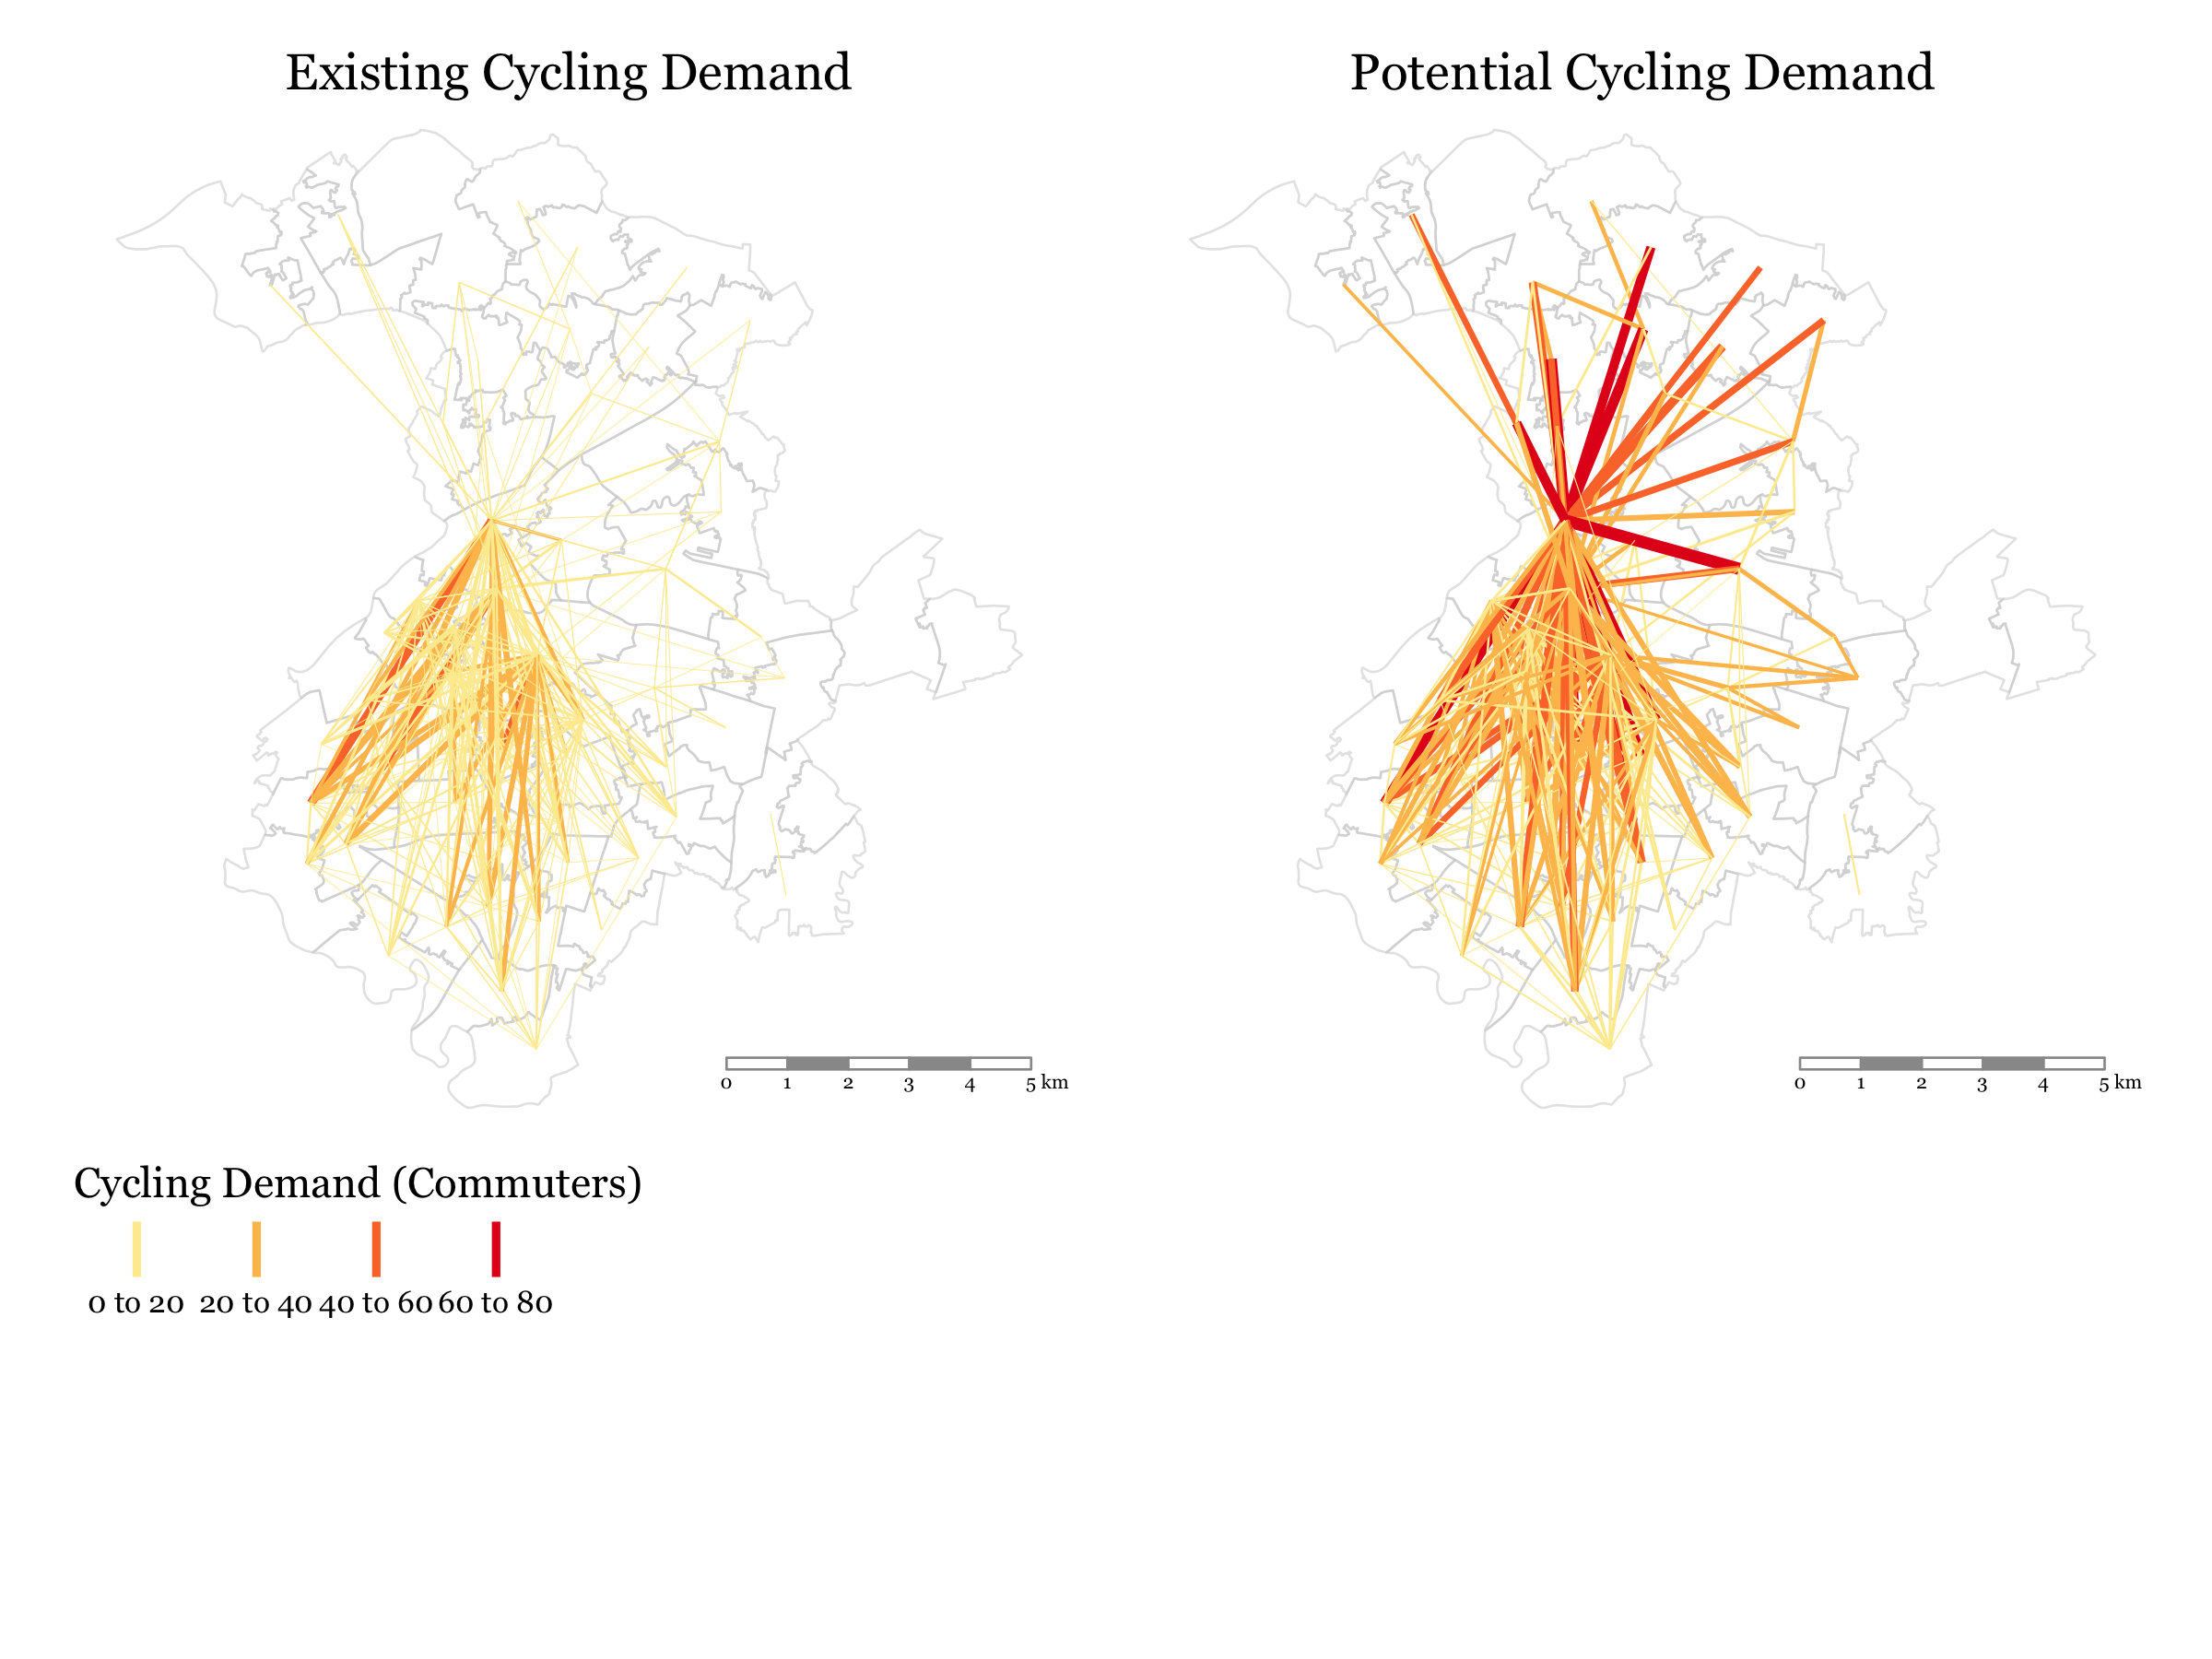
\includegraphics[width=.6\textwidth]{../../data/Manchester/Plots/desire_facet_cycling.png} 
    \caption{Current and Potential Cycling Demand} 
    \label{fig:desire_facet_cycling} 
\end{figure}

\hypertarget{routing}{%
\section{Routing}\label{routing}}

The next step is to route the potential cycling demand
(\(\boldsymbol{C_{p}}\)) between all OD pairs onto the road network.

To conduct routing, the following is considered:

\begin{enumerate}
\def\labelenumi{\arabic{enumi}.}
\tightlist
\item
  \textbf{Cyclist Preference}: Work done by Dill and McNeil (2013) on
  examining cyclist typologies determined that around 60\% of Portland
  residents fit under the \emph{interested but concerned} category.
  These were people that enjoyed cycling but avoided it due safety
  concerns. The key to encouraging this group was to create a low-stress
  cycling network, not only though segregated infrastructure but also by
  planning routes that passed through residential streets.
\item
  \textbf{Low-Traffic Neighborhoods}: The UK Department for Transport is
  allocating funding to local authorities to invest in Active Transport,
  partially through the creation of LTNs (DfT, 2020). This includes
  closing off residential streets to motorized traffic
\item
  \textbf{Existing Cycling Infrastructure}: Utilizing existing cycling
  infrastructure makes economic sense, as small investments may lead to
  large connectivity gains as the disconnected cycling infrastructure
  gets joined together.
\end{enumerate}

The weighting profiles are therefore adjusted to favor less-stressful
streets (based on information from Table \ref{table:osmroadtypes}), and
roads with existing cycling infrastructure. This is also in line with
the creation of LTNs, as residential streets are those where motorized
traffic is most likely to be banned in the creation of LTNs.

\hypertarget{road-segment-prioritization}{%
\section{Road Segment
Prioritization}\label{road-segment-prioritization}}

\begin{figure} [h!]
\centering
\captionsetup{font=footnotesize,labelfont=footnotesize} % size of captions
\begin{subfigure}{.45\textwidth}
  \centering
  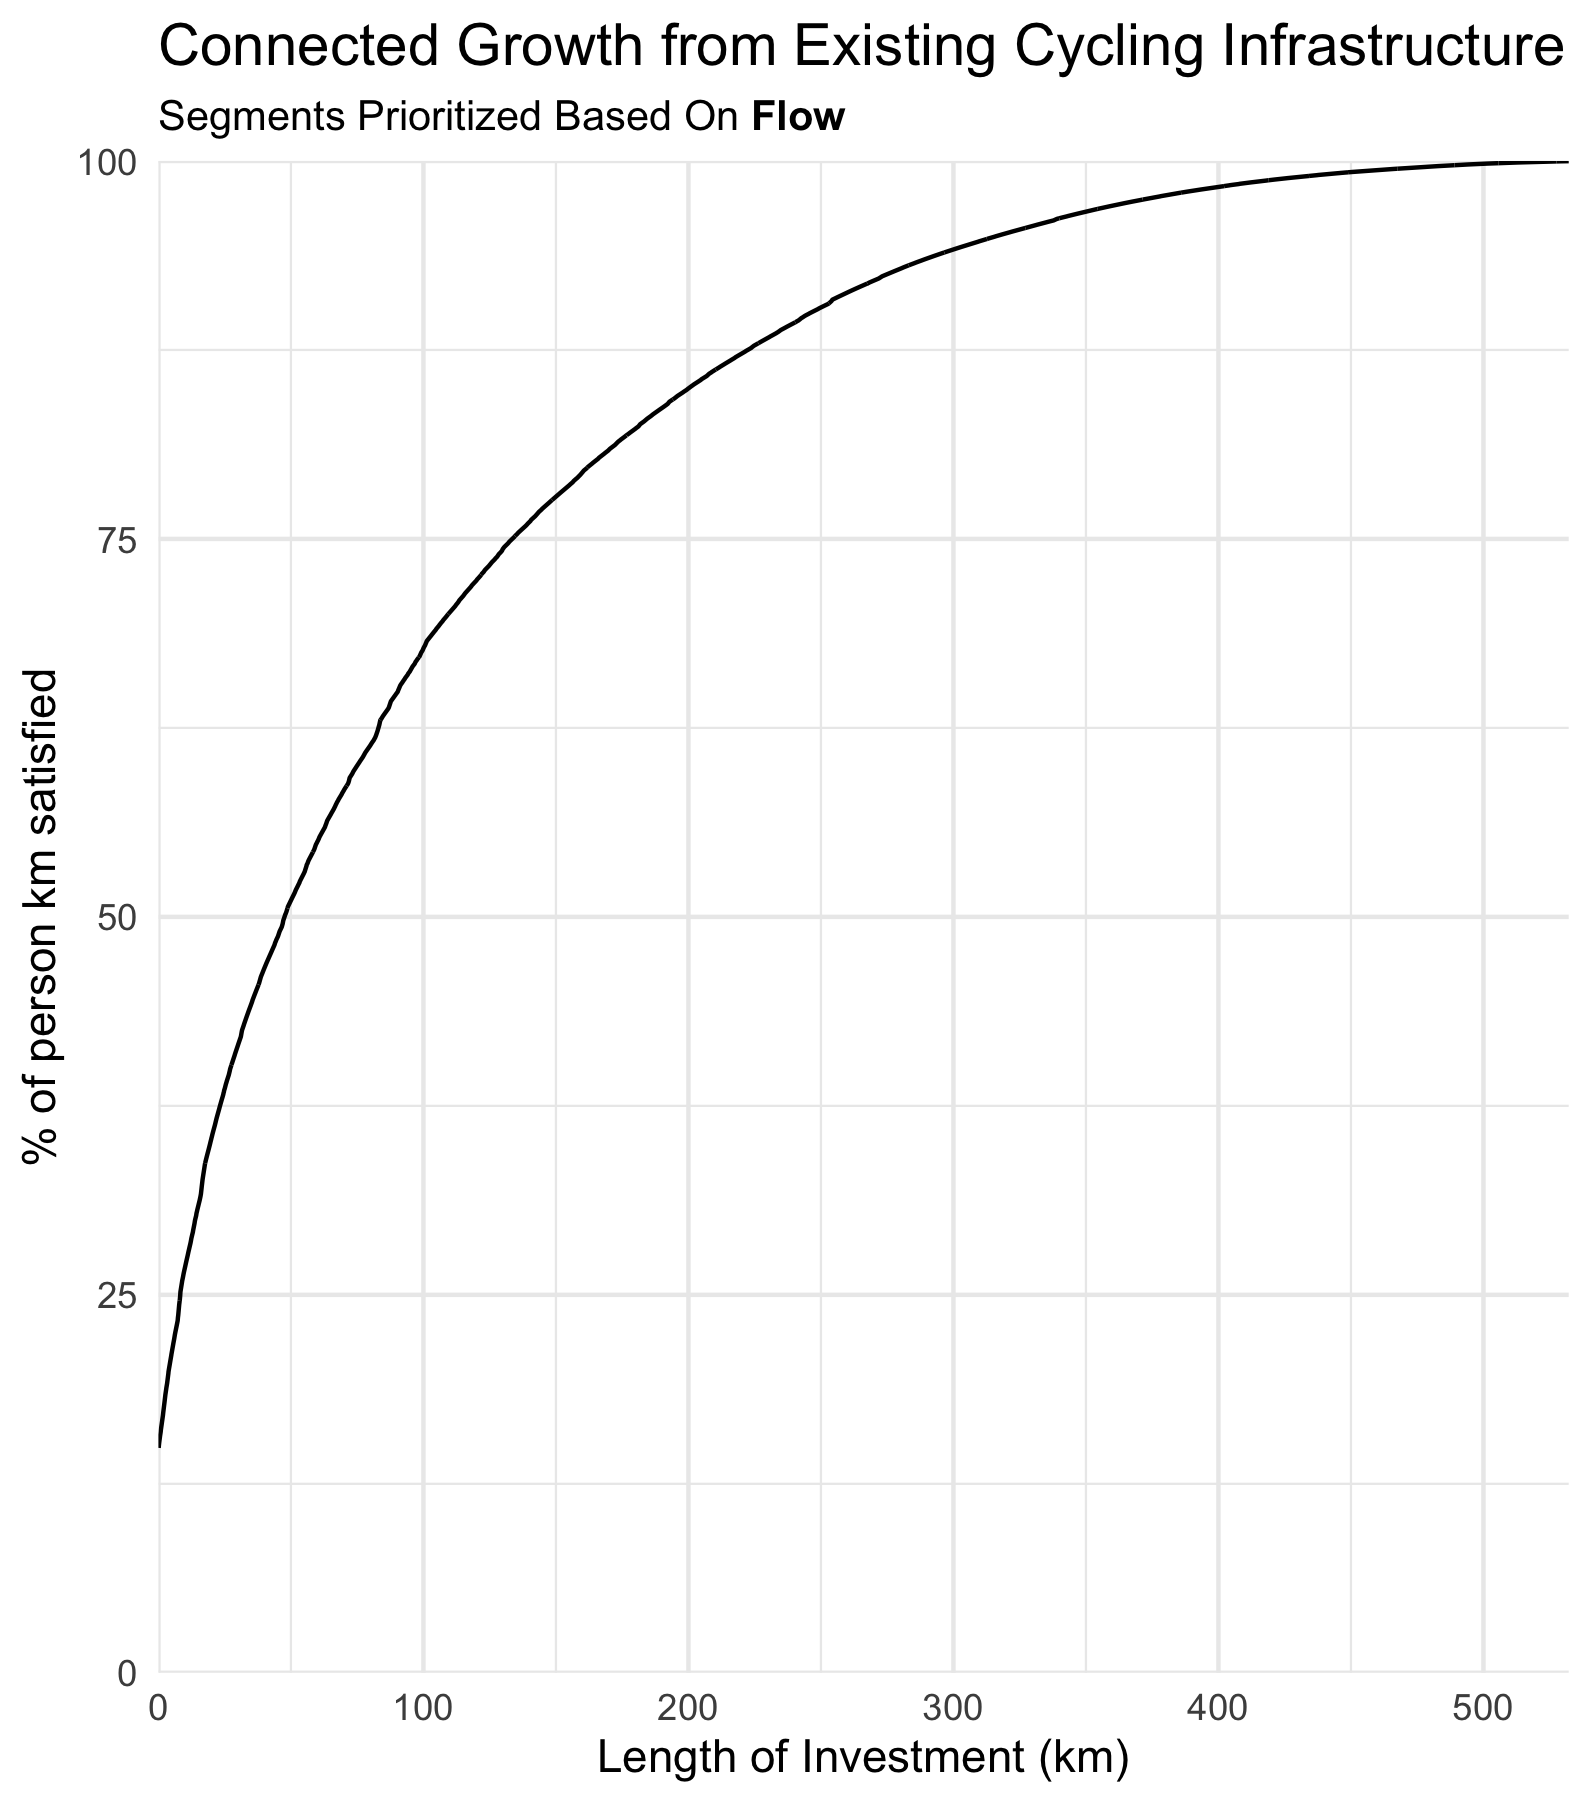
\includegraphics[width=1\linewidth]{../../data/Manchester/Plots/Growth_Results/growth_existing_infra_satisfied_km_all_flow_column.png}
  \caption{Alg 1 (Utilitarian)}
  \label{fig:growth_utilitarian_satisfied_all}
\end{subfigure}
\begin{subfigure}{.45\textwidth}
  \centering
  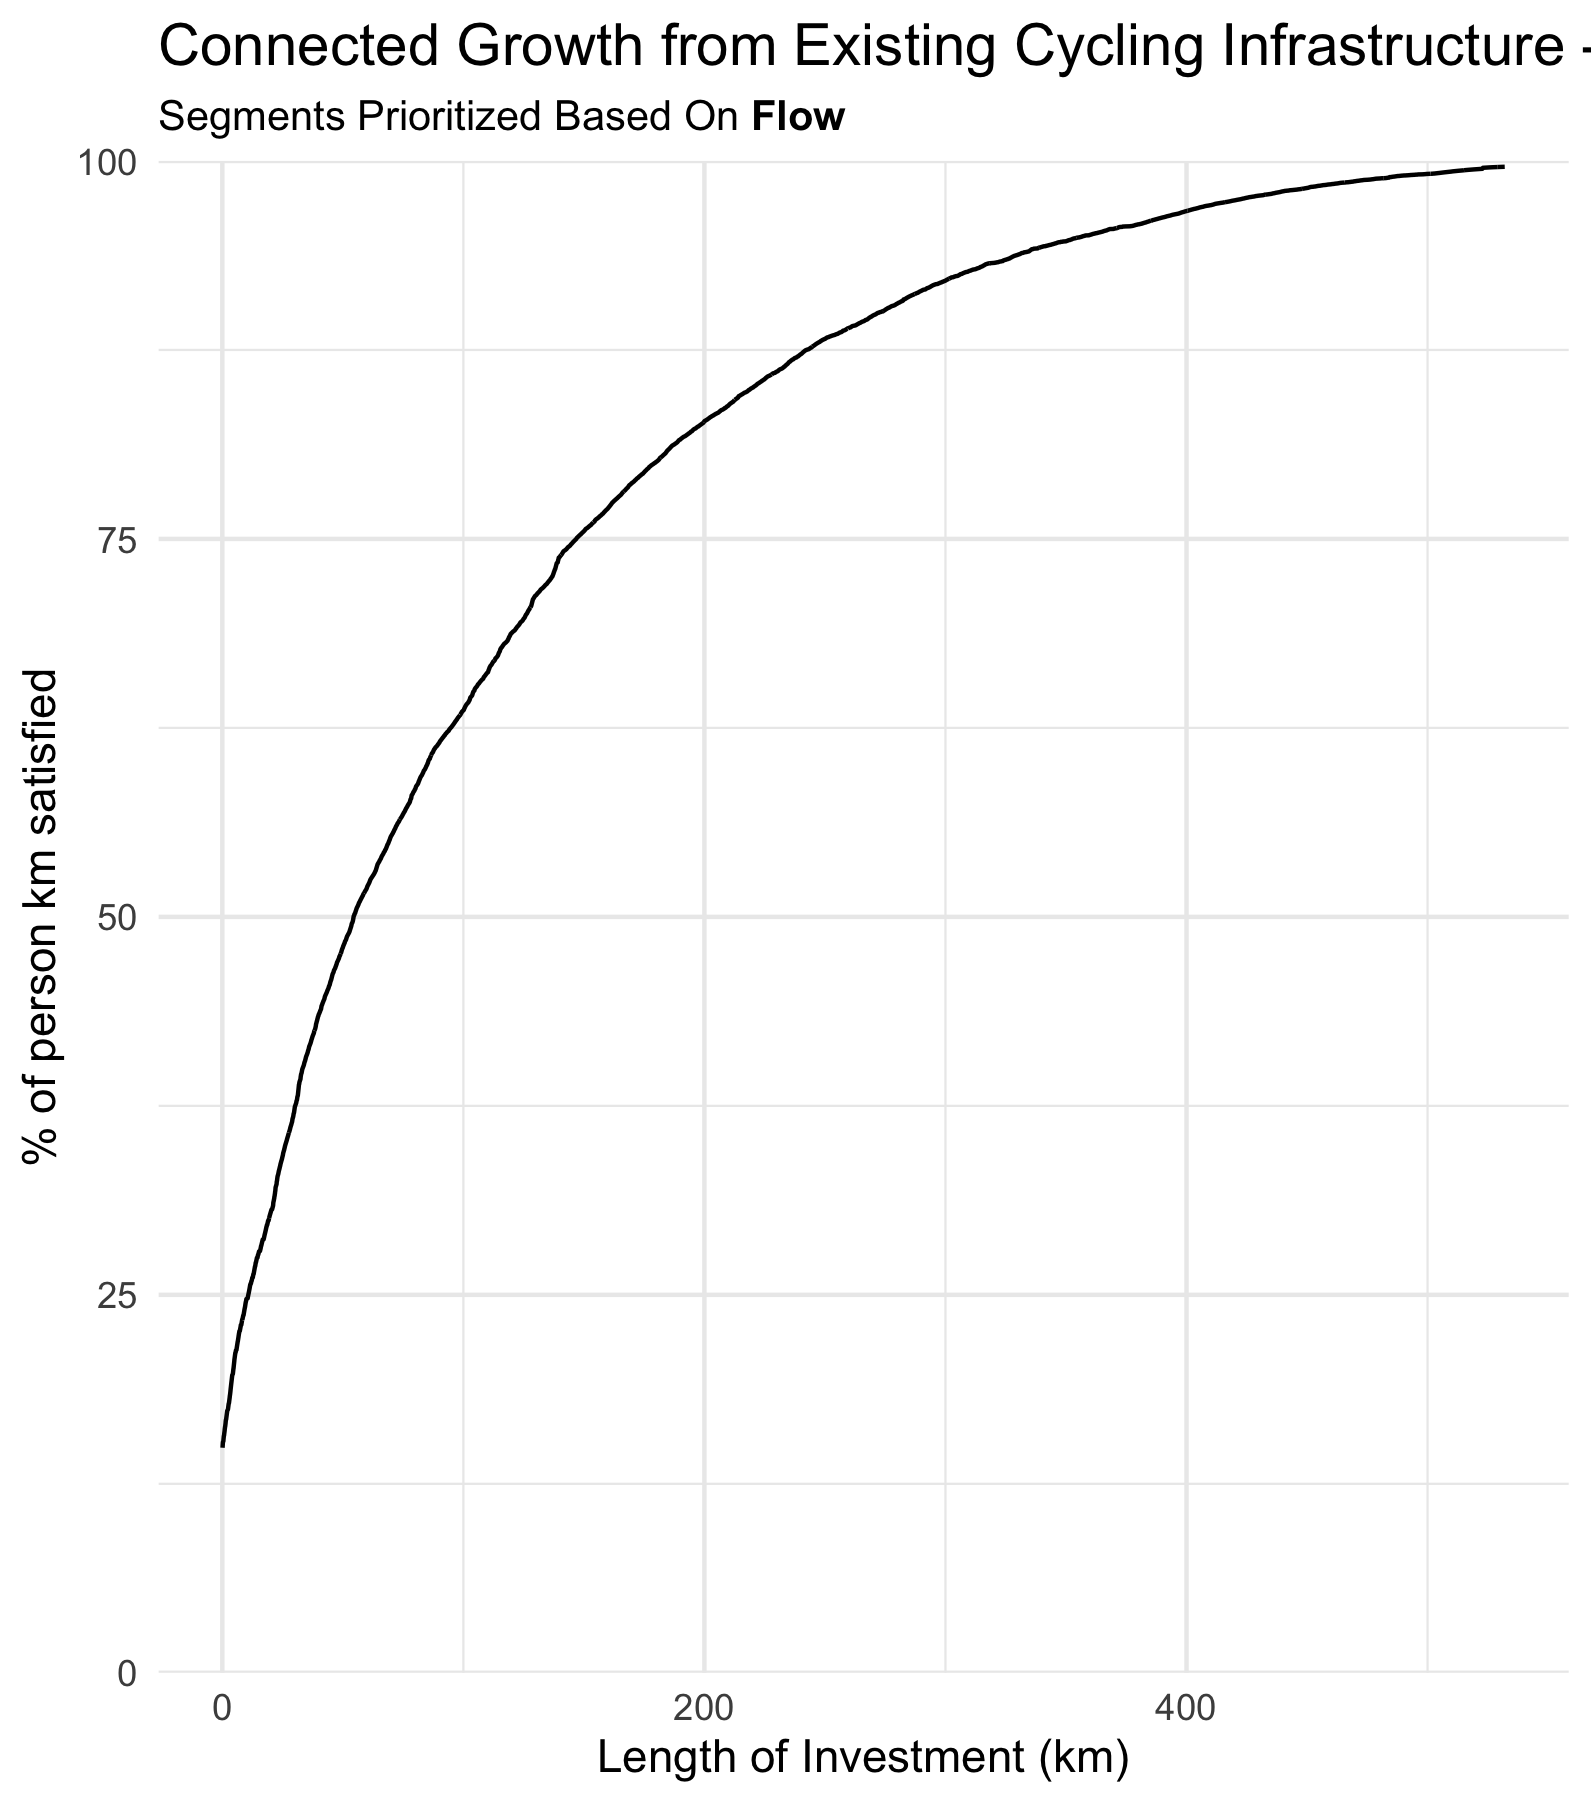
\includegraphics[width=1\linewidth]{../../data/Manchester/Plots/Growth_Results/growth_community_4_satisfied_km_all_flow_column.png}
  \caption{Alg 2 (Egalitarian)}
  \label{fig:growth_egalitarian_satisfied_all}
\end{subfigure}
\caption{Comparing Overall Person-Km Satisfied (Manchester)}
\label{fig:growth_existing_infra_satisfied}
\end{figure}

\hypertarget{overarching-policies}{%
\section{Overarching Policies}\label{overarching-policies}}

While segregated, connected, and direct cycling infrastructure is key to
achieving high levels of cycling, research has shown that it cannot
exist in a vacuum. Wardman et al. (2007) developed a mode choice model
for the UK and their results showed that improved cycling infrastructure
on its own only had modest impacts on mode shift, and even the unlikely
scenario of all urban routes being serviced by segregated bike lanes was
forecast to increase cycling mode share by only 3\%. However, cities
that invest in more comprehensive cycling projects show a more
significant increase in the number of cyclists as well as the cycling
mode share (Pucher et al., 2010). These cities do not just focus on
infrastructure, but on general policies as well as restricting car use.
Evaluation of policies in Denmark and Germany and the Netherlands has
shown that their high cycling mode share is down to a broader set of
policies that also include traffic calming, cycling rights of way, bike
parking, integration with the public transport network, and making
driving cars both expensive and inconvenient (Pucher and Buehler, 2008).
While these policies are outside the scope of this research, it is
important to recognize their key role in bringing about an increase in
levels of cycling.

\hypertarget{conclusions}{%
\section{Conclusions}\label{conclusions}}

\hypertarget{references}{%
\section*{References}\label{references}}
\addcontentsline{toc}{section}{References}

\setlength{\parindent}{-0.5in}
\setlength{\leftskip}{0.5in}
\setlength{\parskip}{8pt}

\hypertarget{refs}{}
\leavevmode\hypertarget{ref-akbarzadeh2018designing}{}%
Akbarzadeh, M., Mohri, S.S., Yazdian, E., 2018. Designing bike networks
using the concept of network clusters. Applied network science 3, 12.

\leavevmode\hypertarget{ref-aldred2019impacts}{}%
Aldred, R., Croft, J., Goodman, A., 2019. Impacts of an active travel
intervention with a cycling focus in a suburban context: One-year
findings from an evaluation of london's in-progress mini-hollands
programme. Transportation research part A: policy and practice 123,
147--169.

\leavevmode\hypertarget{ref-bao2017planning}{}%
Bao, J., He, T., Ruan, S., Li, Y., Zheng, Y., 2017. Planning bike lanes
based on sharing-bikes' trajectories, in: Proceedings of the 23rd Acm
Sigkdd International Conference on Knowledge Discovery and Data Mining.
pp. 1377--1386.

\leavevmode\hypertarget{ref-blondel2008fast}{}%
Blondel, V.D., Guillaume, J.-L., Lambiotte, R., Lefebvre, E., 2008. Fast
unfolding of communities in large networks. Journal of statistical
mechanics: theory and experiment 2008, P10008.

\leavevmode\hypertarget{ref-broach2011bicycle}{}%
Broach, J., Gliebe, J., Dill, J., 2011. Bicycle route choice model
developed using revealed preference gps data, in: 90th Annual Meeting of
the Transportation Research Board, Washington, Dc.

\leavevmode\hypertarget{ref-caulfield2012determining}{}%
Caulfield, B., Brick, E., McCarthy, O.T., 2012. Determining bicycle
infrastructure preferences--a case study of dublin. Transportation
research part D: transport and environment 17, 413--417.

\leavevmode\hypertarget{ref-crane2017longitudinal}{}%
Crane, M., Rissel, C., Standen, C., Ellison, A., Ellison, R., Wen, L.M.,
Greaves, S., 2017. Longitudinal evaluation of travel and health outcomes
in relation to new bicycle infrastructure, sydney, australia. Journal of
Transport \& Health 6, 386--395.

\leavevmode\hypertarget{ref-departmentgearchange2020}{}%
DfT, 2020. Gear change: A bold vision for cycling and walking.

\leavevmode\hypertarget{ref-dill2013four}{}%
Dill, J., McNeil, N., 2013. Four types of cyclists? Examination of
typology for better understanding of bicycling behavior and potential.
Transportation Research Record 2387, 129--138.

\leavevmode\hypertarget{ref-duthie2014optimization}{}%
Duthie, J., Unnikrishnan, A., 2014. Optimization framework for bicycle
network design. Journal of Transportation engineering 140, 04014028.

\leavevmode\hypertarget{ref-goodman2014new}{}%
Goodman, A., Sahlqvist, S., Ogilvie, D., Consortium, 2014. New walking
and cycling routes and increased physical activity: One-and 2-year
findings from the uk iConnect study. American journal of public health
104, e38--e46.

\leavevmode\hypertarget{ref-iacono2010measuring}{}%
Iacono, M., Krizek, K.J., El-Geneidy, A., 2010. Measuring non-motorized
accessibility: Issues, alternatives, and execution. Journal of Transport
Geography 18, 133--140.

\leavevmode\hypertarget{ref-jafino2020transport}{}%
Jafino, B.A., Kwakkel, J., Verbraeck, A., 2020. Transport network
criticality metrics: A comparative analysis and a guideline for
selection. Transport Reviews 40, 241--264.

\leavevmode\hypertarget{ref-lovelace2017propensity}{}%
Lovelace, R., Goodman, A., Aldred, R., Berkoff, N., Abbas, A., Woodcock,
J., 2017. The propensity to cycle tool: An open source online system for
sustainable transport planning. Journal of transport and land use 10,
505--528.

\leavevmode\hypertarget{ref-lucas2016method}{}%
Lucas, K., Van Wee, B., Maat, K., 2016. A method to evaluate equitable
accessibility: Combining ethical theories and accessibility-based
approaches. Transportation 43, 473--490.

\leavevmode\hypertarget{ref-marques2015infrastructure}{}%
Marqués, R., Hernández-Herrador, V., Calvo-Salazar, M., García-Cebrián,
J., 2015. How infrastructure can promote cycling in cities: Lessons from
seville. Research in Transportation Economics 53, 31--44.

\leavevmode\hypertarget{ref-mauttone2017bicycle}{}%
Mauttone, A., Mercadante, G., Rabaza, M., Toledo, F., 2017. Bicycle
network design: Model and solution algorithm. Transportation research
procedia 27, 969--976.

\leavevmode\hypertarget{ref-mesbah2012bilevel}{}%
Mesbah, M., Thompson, R., Moridpour, S., 2012. Bilevel optimization
approach to design of network of bike lanes. Transportation research
record 2284, 21--28.

\leavevmode\hypertarget{ref-nahmias2017integrating}{}%
Nahmias-Biran, B.-h., Martens, K., Shiftan, Y., 2017. Integrating equity
in transportation project assessment: A philosophical exploration and
its practical implications. Transport reviews 37, 192--210.

\leavevmode\hypertarget{ref-natera2019data}{}%
Natera, L., Battiston, F., Iñiguez, G., Szell, M., 2019. Data-driven
strategies for optimal bicycle network growth. arXiv preprint
arXiv:1907.07080.

\leavevmode\hypertarget{ref-olmos2020data}{}%
Olmos, L.E., Tadeo, M.S., Vlachogiannis, D., Alhasoun, F., Alegre, X.E.,
Ochoa, C., Targa, F., González, M.C., 2020. A data science framework for
planning the growth of bicycle infrastructures. Transportation Research
Part C: Emerging Technologies 115, 102640.

\leavevmode\hypertarget{ref-ofn2018population}{}%
ONS, 2018. Population estimates for the uk, england and wales, scotland
and northern ireland: Mid-2017. Hampshire: Office for National
Statistics.

\leavevmode\hypertarget{ref-pereira2017distributive}{}%
Pereira, R.H., Schwanen, T., Banister, D., 2017. Distributive justice
and equity in transportation. Transport reviews 37, 170--191.

\leavevmode\hypertarget{ref-pucher2008making}{}%
Pucher, J., Buehler, R., 2008. Making cycling irresistible: Lessons from
the netherlands, denmark and germany. Transport reviews 28, 495--528.

\leavevmode\hypertarget{ref-pucher2010infrastructure}{}%
Pucher, J., Dill, J., Handy, S., 2010. Infrastructure, programs, and
policies to increase bicycling: An international review. Preventive
medicine 50, S106--S125.

\leavevmode\hypertarget{ref-schoner2014missing}{}%
Schoner, J.E., Levinson, D.M., 2014. The missing link: Bicycle
infrastructure networks and ridership in 74 us cities. Transportation
41, 1187--1204.

\leavevmode\hypertarget{ref-stinson2003commuter}{}%
Stinson, M.A., Bhat, C.R., 2003. Commuter bicyclist route choice:
Analysis using a stated preference survey. Transportation Research
Record 1828, 107--115.

\leavevmode\hypertarget{ref-wardman2007factors}{}%
Wardman, M., Tight, M., Page, M., 2007. Factors influencing the
propensity to cycle to work. Transportation Research Part A: Policy and
Practice 41, 339--350.

\leavevmode\hypertarget{ref-winters2011motivators}{}%
Winters, M., Davidson, G., Kao, D., Teschke, K., 2011. Motivators and
deterrents of bicycling: Comparing influences on decisions to ride.
Transportation 38, 153--168.

\leavevmode\hypertarget{ref-winters2010far}{}%
Winters, M., Teschke, K., Grant, M., Setton, E.M., Brauer, M., 2010. How
far out of the way will we travel? Built environment influences on route
selection for bicycle and car travel. Transportation Research Record
2190, 1--10.

\end{document}
